\section{The Standard Model}

The Standard Model (SM) \cite{Glashow:1961tr, Weinberg:1967tq, Salam:1980jd} is a renormalisable quantum field theory describing the interactions between the elementary constituents of matter through the fundamental forces. The matter particles, described as fields with half-integer spin (fermions), are subdivided in six leptons and six quarks. Leptons and quarks are respectively categorised in three families of particles with the same quantum numbers but with different mass. Each of these particles has an associated antiparticle with the same mass and opposite quantum numbers. 
The fundamental forces are described in terms of exchange of mediator fields with integer spin (bosons). Tables \ref{chp:the:tab:part} and \ref{chp:the:tab:forces} show the elementary particles of the Standard Model, classified as matter particles and force carriers.\par
Matter particles and force carriers obey equations of motion derived from the principle of minimal action from a Lagrangian density. Fermions are described by the free Lagrangian:
\be
\mathcal{L}= \bar{\Psi}(i\gamma^{\mu}\partial_{\mu}-m)\Psi,
\ee

\noindent where $\Psi$ is the fermion field, $\gamma^{\mu}$ are the Dirac matrices and $m$ is the mass of the fermion. Fundamental forces are introduced in the Lagrangian imposing invariance under local transformations  of a given symmetry group. The number of associated boson fields is equal to the number of generators of the symmetry group. The SM Lagrangian is invariant under the gauge group:

\be
SU(3)_{C} \otimes SU(2)_{L} \otimes U(1)_{Y},
\label{chp:theo:eq:gaugegroup}
\ee

\noindent where $SU(3)_{C}$ is the gauge group for strong interactions mediated by gluons, while $SU(2)_{L} \otimes U(1)_{Y}$ is the unified gauge group for electromagnetic and weak interactions mediated by photons, $W^{\pm}$ and $Z$ bosons. \\

\begin{table}[htb!]
\begin{center}
  \begin{tabular}{l c c c c}
  \hline   \hline
   & \multicolumn{2}{c}{Leptons}&\multicolumn{2}{c}{Quarks}\\
   & \multicolumn{4}{c}{Spin 1/2}\\
    Electric charge ($q/e$) & $q=-1$ & $q=0$& $q=+2/3$ & $q=-1/3$\\
  \hline
 I family & $e^{-}$ & $\nu_{e}$ & u & d \\
  Mass & 0.51 \mev& <2 \ev& 2.3 \mev&4.8 \mev\\
  \hline
   II family & $\mu^{-}$ & $\nu_{\mu}$ & c & s \\
  Mass & 105.66 \mev& <2 \ev& 1.275 \gev&95 \mev\\
 \hline
  III family & $\tau^{-}$ & $\nu_{\tau}$ & t & b \\
  Mass & 1.77 \gev& <2 \ev& 173.5 \gev&4.65 \gev\\
  \hline  \hline
\end{tabular}

\captionsetup{width=0.85\textwidth} \caption{\small Table of quark and lepton families with their mass and charge according to the Particle Data Group \cite{Olive:2016xmw}.}
\label{chp:the:tab:part}
\end{center}
\end{table}

\begin{table}[htb!]
\begin{center}
\begin{tabular}{l c c c c c}
  \hline\hline
Force & Electromagnetism & \multicolumn{2}{c}{Weak} & Strong & Gravity\\
Carrier boson & $\gamma$ & W$^{\pm}$ & Z & g($\times$ 8) & G\\
Spin & 1 & 1& 1& 1& 2\\
Electric charge (q/e) & 0 & $\pm$1& 0& 0& 0\\
Mass (\gev) & 0 & 80.385 & 91.1876 & 0& $<6\cdot10^{-35}$\\ 
 \hline \hline
\end{tabular}
\captionsetup{width=0.85\textwidth} \caption{\small Table of gauge bosons in the SM with their mass and charge according to the Particle Data Group \cite{Olive:2016xmw}. Gravity is added for completeness.}
\label{chp:the:tab:forces}
\end{center}
\end{table}


\noindent The SM Lagrangian can be split in two terms,\footnote{This splitting simplifies the discussion, but it introduces a small caveat: the kinetic term of the quarks will be present in both terms even if in the reality there is only a single kinetic term.} one describing strong interactions, known as Quantum Chromodynamics (QCD) and a second one describing electroweak (EW) interactions:

\be
\mathcal{L}_{\rm SM}= \mathcal{L}_{\rm QCD}+\mathcal{L}_{\rm EW}.
\ee

\subsection{Quantum Chromodynamics}

The introduction of the strong interaction arose from the need to explain what keeps protons together inside nuclei and quarks bound inside hadrons. The postulation of colour as fundamental charge of the strong interaction was motivated by the need to achieve a description of the $\Delta^{++}$ baryon consistent with Fermi-Dirac statistics. Being a spin-3/2 fermion composed of three identical quarks ($uuu$), an additional feature was required in order to build a wavefunction fully antisymmetric under the interchange of quarks. At the same time, an explanation was needed for the lack of experimental observations of free quarks or $qq$ states. The proposed solution was the existence of a new quantum number, $C$, the colour charge with three different possible values: red (R), blue (B) and green (G). A quark can carry one colour at the time, while anti-quarks carry anti-colours. Only colour-singlet states exist as bound states. The carriers of the strong interaction, called gluons, are massless spin-1 bosons, carrying one of eight bi-colour combinations, i.e. a superposition of colour-anti-colour states, but no electric charge. \par
Quantum ChromoDynamics (QCD) is a gauge theory of strong interactions between quarks and gluons based on the symmetry group $SU(3)_{C}$. Quarks are colour triplets and for each flavour three fields with different colour index ($i$) are present, $q_{i}$. Under a local gauge $SU(3)_{C}$ transformation, the quark field $q$ transforms as follows:

\be
q \to q^{\prime} = e^{ig_S T_a \cdot \theta^{a}(x)}q, \,\, \textrm{with $a$=1,...,8 ,} 
\ee

\noindent where $\theta_{a}(x)$ is an arbitrary phase that is a-priori different for each point in space-time, $T_a=\frac{\lambda_{a}}{2}$ refers to the group generators of $ SU(3)_{C}$, with $\lambda_{a}$ being the eight Gell-Mann matrices, which are 3$\times$3 generalisations of the Pauli matrices, and $g_{s}=\sqrt{4\pi\alpha_{s}}$ is the strong coupling. The group is non-abelian and the commutation rules are the following:
\be
\left [T_a , T_b \right ] = i f_{abc} T_c,
\ee
\noindent where $f_{abc} $ are the structure constants of the group. To ensure the local gauge invariance of the Lagrangian the covariant derivative is introduced:
\be
D_{\mu}\equiv \partial_{\mu}+ig_{s}T_{a}G_{\mu}^{a},
\ee
\noindent where $G_{\mu}^{a}$ are the gluon fields, which transform as $G_{\mu}^{a}\to G_{\mu}^{a~\prime}=G_{\mu}^{a}-\frac{1}{g_s}\partial_{\mu}\theta^{a}$ . The interactions between quarks and gluons are enclosed in the definition of the covariant derivative.\par
After introducing the covariant derivative and a kinetic term for the gluon fields, the QCD Lagrangian is given by:

\be
\mathcal{L}_{\rm QCD} = \bar{q}(i\gamma^{\mu}D_{\mu} - m)q -\frac{1}{4} G_{\mu \nu}^{\alpha} G^{\mu \nu}_{\alpha},
\ee

\noindent where the $G_{\mu \nu}^{\alpha}$ tensor field is defined as:

 \be
G_{\mu \nu}^{\alpha} = \partial_{\mu} G_{\nu}^{a}-\partial_{\nu} G_{\mu}^{a}-g_{s}f_{abc} G_{\mu}^{b}G_{\nu}^{c}.
\label{chp:theo:eq:gluontensor}
\ee

Being carriers of colour charge, gluons can self-interact. This self-interaction is described by the third term of equation \ref{chp:theo:eq:gluontensor} and has an effect on the way the strong coupling evolves as a function of the energy scale $Q$ at which the interaction takes place.
At the leading order (LO), the strong coupling constant can be expressed as:

\be
\alpha_{s}(Q^{2})=\frac{12\pi}{(33-2n_{f})\log\left(Q^{2}/\Lambda^{2}_{\rm QCD}\right)},
\ee
\noindent where $n_{f}$ is the number of  active quark flavours (i.e. with $m_{q}<Q$) and $\Lambda_{\rm QCD}$ is an infrared cut-off scale ($\Lambda_{\rm QCD} \sim 200$ $\mev$) below which the perturbative approximation is no longer valid. The strong coupling constant is decreasing with increasing energy (or decreasing distance), as shown in figure \ref{sec:theo:fig:alpha}.

\bfig[h!]
\centering
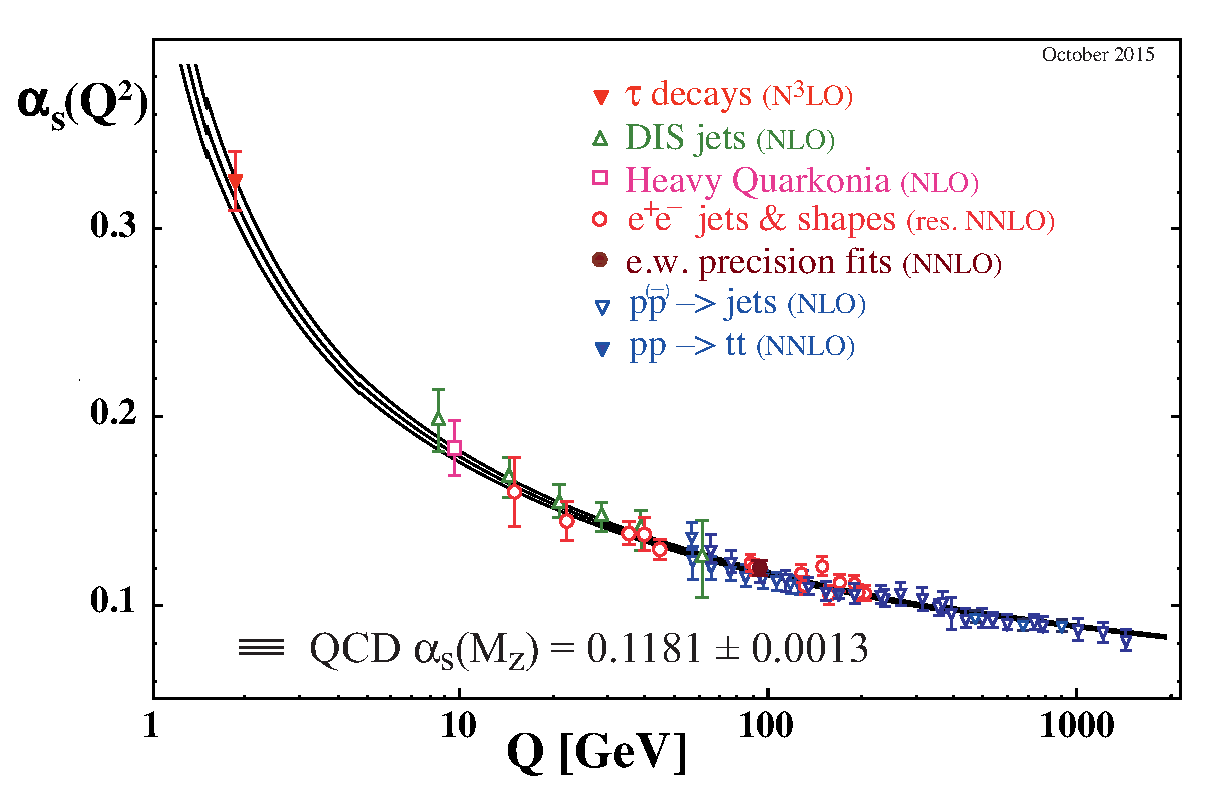
\includegraphics[width=0.6\textwidth]{figures/Theory/asq-2015.eps}
\captionsetup{width=0.85\textwidth} \caption{\small Evolution of the strong coupling constant $\alpha_s$ with energy scale $Q$, as probed by different measurements. From reference \cite{Bethke:2015etp}.}
\label{sec:theo:fig:alpha}
\efig


In the high-energy (i.e. short-distance) regime, $\alpha_{s}$ is sufficiently small that perturbation theory fully applies, and asymptotically quarks and gluons can be considered as free particles. This property is referred to as ``asymptotic freedom'' \cite{Politzer:1973fx,Gross:1973id}, and it is particularly important for the computability of cross sections at hadron colliders.
On the other hand, at lower energies (i.e. longer distances) $\alpha_{s}$ increases to the point of diverging; i.e. quarks and gluons cannot be found as free particles. This property is known as ``confinement'': when trying to separate two quarks, the potential energy increases enough that a quark-antiquark pair is created from the vacuum and colorless hadrons are eventually formed. Therefore, quarks and gluons produced as the result of interactions among particles at high energy will manifest themselves in the detector as collimated sprays of colorless hadrons called ``jets''.
At low energies ($Q<\Lambda_{\rm QCD}$), where the perturbative approximation is no longer valid, numerical (lattice QCD) or phenomenological (hadronisation models) approaches have to be used in order to describe this regime.

\subsection{Electroweak theory}

The gauge invariance of electromagnetism was already introduced in Maxwell's formulation of Electrodynamics \cite{maxwell1873treatise}. It was later extended to the invariance under a local phase transformation, which accommodated the explanation of the interaction in terms of Quantum ElectroDynamics (QED). The weak interaction was first identified by studying $\beta$-decays of atomic nuclei in the late 19th century. The experiments regarding these decays also lead to the postulation of neutrinos by Wolfgang Pauli \cite{Pauli:83286}, introduced to ensure the energy, momentum and spin conservation in these processes. After the parity violation of the weak processes was confirmed in the experiment conducted by C.-S. Wu \cite{Wu:1957my}, a new gauge theory formulation was constructed. The Wu experiment showed that the decay particles were travelling in a direction opposite to their spin, which suggested that the weak interaction had a form of a difference of a vector (representing the particle momentum) and an axial vector (representing the particle spin), i.e. a V-A form. The weak interaction is thus not the same for a particle and its mirror symmetric partner. This feature is referred to as the parity violation (P violation) of the weak interaction. It was shown later that the weak interaction violates as well the CP (charge conjugation and parity) symmetry \cite{Wolfenstein:1964ks} and the T (time reversal) \cite{Lees:2012uka}, but conserves CPT \cite{Lee:1965js}.\par
The electroweak theory describes the weak and the electromagnetic interactions, using a Lagrangian invariant under transformations of the symmetry group $SU(2)_{L} \otimes U(1)_{Y}$. The $SU(2)_{L}$ group introduces the weak isospin quantum number ($T$). The group is non-abelian and the commutation rules for the generators of the group are the following:
\be
\left [T_i , T_j \right ] = i \epsilon_{ijk} T_k,
\ee
\noindent where $\epsilon_{ijk}$ is the totally-antisymmetric Levi-Civita tensor and $T_i=\frac{\sigma_i}{2}$ $(i=1,2,3)$, where $\sigma_i$ are the Pauli matrices. Three bosons are introduced for $SU(2)_{L}$ according to the number of group generators. The fermions have different $SU(2)_{L}$ representation according to their chiral structure, defined as $f_{L,R}=\frac{1}{2}(1\mp \gamma_{5})f$, with $\gamma_{5}= i \gamma_{0}\gamma_{1}\gamma_{2}\gamma_{3}$. Left-handed fermions are weak-isospin doublets ($T_{3}=\pm1/2$) while right-handed fermions are singlets ($T_{3}=0$), where $T_{3}$ is the third component of the weak isospin. Only left-handed components participate in weak interaction, thus explaining the subscript in $SU(2)_{L}$. The abelian group $U(1)_{Y}$ introduces the hypercharge quantum number, $Y$, defined using the Gell-Mann-Nishijima formula:
\be
Q = T_{3}+\frac{Y}{2},
\ee

\noindent where $Q$ is the electric charge. \noindent Electric charge and hypercharge are quantities absolutely conserved.\\ Table \ref{chp:the:tab:particles} shows the multiplets of fermions fields and their $T$, $T_{3}$, $Y$ and $Q$ quantum numbers.

\begin{table}[t!]
\begin{center}
  \begin{tabular}{|c||c c c||c|c|c|c|}
  \hline
  & \multicolumn{3}{c}{Fermions multiplets}&$T$&$T_{3}$&$Y$&$Q$\\
     \hline \hline
    \multirow{2}{*}{Leptons}&$\begin{pmatrix} e\\ \nu_{e}\\ \end{pmatrix}_{L}$&$\begin{pmatrix} \mu\\ \nu_{\mu}\\ \end{pmatrix}_{L}$&$\begin{pmatrix} \tau\\ \nu_{\tau}\\ \end{pmatrix}_{L}$&$1/2$&$\begin{matrix}+1/2\\-1/2\\ \end{matrix}$&$-1$&$0$\\
    &$e_{R}$&$\mu_{R}$&$\tau_{R}$&0&0&$-2$&$-1$\\
\hline
 \multirow{3}{*}{Quarks}&$\begin{pmatrix} u\\ d^{\prime}\\ \end{pmatrix}_{L}$&$\begin{pmatrix} c \\ s^{\prime}\\ \end{pmatrix}_{L}$&$\begin{pmatrix} t \\ b^{\prime}\\ \end{pmatrix}_{L}$&$1/2$&$\begin{matrix}+1/2\\-1/2\\ \end{matrix}$&$+1/3$&$\begin{matrix}+2/3\\-1/3\\ \end{matrix}$\\
    &$u_{R}$&$c_{R}$&$t_{R}$&0&0&+4/3&+2/3\\
    &$d_{R}$&$s_{R}$&$b_{R}$&0&0&$-2/3$&$-1/3$\\
  \hline
\end{tabular}

\captionsetup{width=0.85\textwidth} \caption{\small Weak isospin multiplets. Here $d^{\prime}$, $s^{\prime}$, and $b^{\prime}$ denote flavour eigenstates, each of which can be expressed as a linear combination of the mass eigenstates ($d$, $s$, and $b$) weighted by CKM matrix elements \cite{cab,ckm}.}
\label{chp:the:tab:particles}
\end{center}
\end{table}


Under a local gauge transformation of the $SU(2)_{L} \otimes U(1)_{Y}$ group a fermionic field $\Psi(x)$ transforms as:
\be
\Psi(x) \to \Psi^{\prime}(x) = e^{\frac{i}{2}\vec{\sigma}\cdot \vec{\alpha}(x)}e^{i\frac{Y}{2}\beta(x)}\Psi(x).
\ee

\noindent To ensure local gauge invariance of the lagrangian the covariant derivative is introduced:
\be
D_{\mu}^{L}\equiv \partial_{\mu}+ig T_{i} W_{\mu}^{i}+ig^{\prime}\frac{Y}{2}B_{\mu}, \,\,\,\,\,\,\,\,
D_{\mu}^{R}\equiv \partial_{\mu}+ig^{\prime}\frac{Y}{2}B_{\mu} ,
\label{chp:theo:eq:EWderivative}
\ee
\noindent where $D_{\mu}^{L}$ acts on weak-isospin doublets and $D_{\mu}^{R}$, instead, on singlets. The coupling constants $g$ and $g^{\prime}$ are associated with the $SU(2)_{L}$ and $U(1)_{Y}$ gauge groups respectively, and $W_{\mu}^{i}$, $B_{\mu}$ denote the gauge fields of the respective gauge groups. The $SU(2)_{L}$ gauge fields transform as $\vec W_{\mu} \to \vec W_{\mu} -\frac{1}{g}\partial_{\mu} \vec \alpha - \vec \alpha\times \vec W_{\mu} $, while the $U(1)_{Y}$ gauge field transforms as  $B_{\mu}\to B_{\mu} -\frac{1}{g^{\prime}}\partial_{\mu}\beta$. \par
After introducing the covariant derivative and a kinetic term for the gauge fields, the EW Lagrangian is:
\be
\mathcal{L}_{\rm EW} = i \bar{f_{L}}\gamma^{\mu}D_{\mu}^{L}f_{L}+ i \bar{f_{R}}\gamma^{\mu}D_{\mu}^{R}f_{R} -\frac{1}{4} W_{\mu \nu}^{i} W^{\mu \nu}_{i} -\frac{1}{4} B_{\mu \nu} B^{\mu \nu},
\label{chp:the:eq:LEW}
\ee
\noindent where $i=1,2,3$, and $W_{\mu \nu}^{i}$ and $B_{\mu \nu}$ are the field tensors for $SU(2)_{L}$ and $U(1)_{Y}$ respectively, defined as:
\be
W_{\mu \nu}^{i}=  \partial_{\mu} W_{\nu}^{i}-\partial_{\nu} W_{\mu}^{i}-g\epsilon_{ijk} W_{\mu}^{j}W_{\nu}^{k}, \,\,\,\,\,\,\,\,
B_{\mu \nu}=  \partial_{\mu} B_{\nu}-\partial_{\nu} B_{\mu}.
\ee
The introduction of mass terms for gauge fields ($\frac{1}{2}M_{V}^{2}W_{\mu}W^{\mu}$) or fermion fields ($-mf_{L}f_{R}$) in equation \ref{chp:the:eq:LEW} would violate the local gauge invariance under $SU(2)_{L} \otimes U(1)_{Y}$, since those terms couple left- and right-handed components. 
Breaking gauge invariance would consequently break the renormalisability of the SM. Therefore, a mechanism for generating non-zero masses while preserving the renormalisability of the theory needs to be introduced to be consistent with the experimental observation of massive fermions and vector bosons.

\subsection{The Brout-Higgs-Englert mechanism}

The Brout-Higgs-Englert (BEH) mechanism \cite{HiggsOriginal2,HiggsOriginal,Higgs:1964ia,Guralnik:1964eu} solves the apparent contradiction between massive particles and the requirement of gauge invariance. This mechanism triggers a Spontaneous Symmetry Breaking (SSB), $SU(2)_{L} \otimes U(1)_{Y} \to U(1)_{\rm EM}$, where $U(1)_{\rm EM}$ denotes the gauge group describing electromagnetism. The SSB is triggered by introducing a complex scalar field. This field, referred to as ``Higgs field'', must have the form of a $SU(2)_{L} \otimes U(1)_{Y}$ multiplet in order to satisfy the SM gauge invariance. In the so called ``minimal'' Higgs sector, the Higgs field is an $SU(2)_{L} \otimes U(1)_{Y}$-isodoublet with isospin $T =1/2$ and the hypercharge $Y= 1$:

\be
\Phi=\begin{pmatrix} \phi^{+}\\ \phi^{0}\\ \end{pmatrix},
\ee

\noindent containing one positively-charged component $\phi^{+}$ and one neutral component $\phi^{0}$. \par
The dynamics of this field, which will be added to the $\mathcal{L}_{\rm EW}$, is given by the Lagrangian:

\be
\mathcal{L}_{\rm Higgs}=(D_{\mu}\Phi)^{\dagger}D^{\mu}\Phi -V(\Phi),
\ee

\noindent where $D_{\mu}$ is the covariant derivative (see equation \ref{chp:theo:eq:EWderivative}) and the potential $V(\Phi)$ is:

\be
 V(\Phi)=\mu^{2}\Phi^{\dagger}\Phi+\lambda(\Phi^{\dagger}\Phi)^{2}.
 \ee

In order for $V(\Phi)$ to have at least one stable minimum $\lambda$ is required to be positive. For $\lambda>0$, two possibilities arise: $\mu^{2}>0$ and $\mu^{2}<0$, which are illustrated in figure \ref{fig:theo:higgspotential}. 
\begin{figure}[h!]
\begin{subfigure}{0.5\textwidth}
  \centering
  \includegraphics[width=0.9\textwidth]{figures/Theory/higgs1.eps}
  \caption{}
  \label{fig:theo:higgs1}
\end{subfigure}
\begin{subfigure}{0.5\textwidth}
  \centering
  \includegraphics[width=0.9\textwidth]{figures/Theory/higgs2.eps}
  \caption{}
  \label{fig:theo:higgs2}
\end{subfigure}

\captionsetup{width=0.85\textwidth} \caption{\small Vacuum potential for $\lambda>0$ and (a) $\mu^{2}>0$ or (b) $\mu^{2}<0$, with the typical shape of a Mexican hat.}
\label{fig:theo:higgspotential}
\end{figure}
In the first case, $\mu^{2}>0$, there is a single solution to the minimisation which corresponds to $|\Phi|= 0$ and provides a vacuum expectation value (VEV), $\langle \Phi \rangle_{0}=\langle 0|\Phi|0 \rangle= 0$. If $\mu^{2}<0$, there is no unique minimum with a VEV, $\langle \Phi \rangle_{0}=\langle 0|\Phi|0 \rangle= v/\sqrt{2}$ and the potential $V(\Phi)$ presents a ``Mexican hat'' shape (figure \ref{fig:theo:higgs2}) with its minimum at:
\be
\Phi^{\dagger}\Phi=-\frac{\mu^{2}}{2\lambda}=\frac{v^{2}}{2},
\ee

\noindent where $v=\sqrt{-\mu^{2}/\lambda}$. In this case, the fundamental vacuum state is no longer invariant
under $SU(2)_{L} \otimes U(1)_{Y}$, meaning that these two symmetries are now broken. When a continuous symmetry is broken Goldstone bosons,  massless scalars, are present (Goldstone theorem \cite{PhysRev.127.965}) and they can be absorbed by a gauge field as a longitudinal polarisation component, resulting in the gauge field acquiring mass. Since the photon is the only electroweak boson known to be massless, the minimum of the potential is chosen so that the Higgs field that acquires a VEV is the one with zero electric charge in order to not break $U(1)_{\rm EM}$:

\be
\Phi_{0}=\frac{1}{\sqrt{2}}\begin{pmatrix} 0\\ v\\ \end{pmatrix}.
\ee

\noindent An infinitesimal $SU(2)_{L}$ transformation around the vacuum can then be expressed as:

\be
\Phi^{\prime}(x)=\frac{e^{i\vec \sigma\cdot \vec \theta(x)/v}}{\sqrt{2}}\begin{pmatrix} 0\\ v + H(x)\\ \end{pmatrix},
\ee

\noindent with $H(x)$ denoting a real scalar field associated to a physical degree of freedom, the Higgs-boson particle, and $\theta$ denoting the three fields which will be absorbed by the gauge fields.
With this choice of the vacuum and the gauge, the Lagrangian of the physical Higgs field reads:

\be
\mathcal{L}_{\rm Higgs}=(D_{\mu}H)^{\dagger}D^{\mu}H -\frac{1}{2}(-2\mu^{2})H^{2}-\lambda v H^{3}-\frac{1}{4}\lambda H^{4},
\ee

\noindent where the second term corresponds to the tree-level mass term of the $H(x)$ field, $m_{H}=\sqrt{-2\mu^{2}}=\sqrt{2\lambda}v$, and the last two terms describe interactions among Higgs fields. Since the value of $\lambda$  is unknown, $m_{H}$ is not predicted by the theory and must be determined experimentally.\par
Furthermore, this procedure has also generated the masses of the gauge bosons. This becomes obvious from the development of $|D_{\mu}\Phi^{\prime}|^{2}$, which provides terms of the form:

\begin{equation}
  \begin{split}
    & \left|\left(-ig\frac{\vec \sigma}{2}\vec{W}_\mu - i\frac{g'}{2}B_\mu \right)\Phi\right|^2 
    = \frac{1}{8} \left|\left(
    \begin{matrix}
      gW_\mu^3 + g'B_\mu & g(W_\mu^1 - iW_\mu^2) \\
      g(W_\mu^1 + iW_\mu^2) & -gW_\mu^3 + g'B_\mu 
    \end{matrix}
    \right)
    \left(
    \begin{matrix}
      0 \\%
      v   \
    \end{matrix}
    \right) \right|^2 \\
    &= \frac{1}{8} v^2 g^2 \left[(W_\mu^1)^2 + (W_\mu^2)^2\right] + \frac{1}{8} v^2 (g'B_\mu - gW_\mu^3)(g'B^\mu - gW^{3\mu}) \\
    &= \left(\frac{1}{2}vg\right)^2 W_\mu^{+} W^{-\mu} + \frac{1}{8} v^2 \left(W_\mu^3, B_\mu\right) 
    \left(
    \begin{matrix}
      g^2 & -gg' \\
      -gg' & g'^2
    \end{matrix}
    \right)
    \left(
    \begin{matrix}
      W_\mu^3 \\
      B_\mu
    \end{matrix}
    \right),
  \end{split}
  \label{eq:HiggsBosonMassDemonstration}
\end{equation}

\noindent defining the charged fields as $W^{\pm} = (W^1 \mp iW^2)/\sqrt{2}$. The mass eigenstates can be obtained diagonalizing the mass matrix, and expressed as a function of $W_\mu^3$ and $B_\mu$:

\begin{equation}
\begin{split}
    \frac{1}{8}v^2\left[g^2\left(W_\mu^3\right)^2 - 2gg'W_\mu^3 B^\mu + g'^2B_\mu^2\right] 
    =\ & \frac{1}{8}v^2\left[ gW_\mu^3 - g'B_\mu\right]^2           \\
    &+ 0 \left[g'W_\mu^3 + gB_\mu\right]^2 \\
    =\ & \frac{1}{2}\left(v\frac{\sqrt{g^2+g'^2}}2\right)^2 Z_\mu^2 \\
    &+ 0 \cdot A_\mu^2, 
\end{split}
  \label{eq:HiggsBosonMassDemonstration2}
\end{equation}

\noindent where $Z_\mu$ and $A_\mu$  can be defined as:

\begin{equation}
  Z_\mu = \frac{gW_\mu^3 - g'B_\mu}{\sqrt{g^2 + g'^2}}= \cos \theta_{W} W^{3}_{\mu}-\sin \theta_{W} B_\mu,
  \label{eq:HiggsZdefinition}
\end{equation}
\begin{equation}
  A_\mu = \frac{g'W_\mu^3 + gB_\mu}{\sqrt{g^2 + g'^2}}=\sin \theta_{W} W^{3}_{\mu}+\cos \theta_{W} B_\mu,
  \label{eq:HiggsAdefinition}
\end{equation}
\noindent representing the fields associated with the $Z$ boson and the photon respectively, and $\theta_{W}$ is the Weinberg angle, $\tan \theta_W = g^{\prime}/g$.
From equations \ref{eq:HiggsBosonMassDemonstration} and \ref{eq:HiggsBosonMassDemonstration2}, the tree level predictions for masses of the gauge bosons and the relation between the coupling constants can be derived:

\be
 m_W = \frac{vg}{2}=m_Z \cos \theta_{W}, 
\ee

\be
m_Z = v \frac{\sqrt{g^2 + g'^2}}{2},
\ee
\be
 m_\gamma = 0.
 \ee


The BEH mechanism can provide as well mass to the fermions, by postulating their coupling to the Higgs boson via a Yukawa interaction:

\be
\mathcal{L}_{\rm Yukawa}=\displaystyle\sum_{f=\ell,q}y_{f}\left[ \bar{f}_{L}\Phi f_{R}+\bar{f}_{R}\bar{\Phi} f_{L}\right],
\label{chp:theo:eq:yukawa}
\ee

\noindent where the matrices $y_{f}$ describe the Yukawa couplings between the Higgs doublet and the fermions. The Yukawa Lagrangian is gauge invariant since the combinations $\bar{f}_{L}\Phi f_{R}$ and $\bar{f}_{R}\bar{\Phi} f_{L}$ are $SU(2)_{L}$ singlets. The $y_{f}$ matrices can be diagonalised to obtain the eigenvalues of the Yukawa couplings using unitary transformations that will redefine the fermion fields. In the leptonic sector this transformation has no effect given the absence of right-handed neutrinos, while in the quark sector, the rotation to the mass eigenstate basis introduces a mixing among fermion families that is manifest in the weak interactions. The mixing between the weak eigenstates of the down-type quarks,\footnote{By convention, the mixing takes place between down-type quarks only, while the up-type mass matrix is diagonal.} $d^{\prime}$, $s^{\prime}$ and $b^{\prime}$, and the corresponding mass eigenstates $d$, $s$ and $b$, is described by the Cabibbo-Kobayashi-Maskawa (CKM) matrix \cite{ckm}. Off-diagonal elements of the CKM matrix have the result that $W$ bosons can couple to two quark belonging to two different families. The CKM matrix is fully specified by four parameters: three mixing angles controlling the mixing between each family pair and one complex phase responsible for CP-violating phenomena.\par
The tree-level predictions for the mass of the fermions are obtained introducing the expansion of the Higgs doublet in equation \ref{chp:theo:eq:yukawa}:

\be
m_{f}=\frac{y_{f}v}{\sqrt{2}}.
\ee

\noindent While the gauge-boson masses can be determined from the known values of the coupling constants $g$ and $g^{\prime}$, the fermion masses are free parameters, since their Yukawa couplings $y_{f}$ are not predicted by the SM. 


\subsection{Higgs boson production and decay in the Standard Model}

The most important production modes for the SM Higgs boson at the LHC are displayed in figure \ref{fig:theo:higgsprod}, with their cross sections shown in figure \ref{fig:theo:higgsxsec}.
The dominant production mechanism is gluon-gluon fusion (ggF) mediated by a virtual quark loop, where the main contribution is from the top quark, owing to its large Yukawa coupling.
The ggF production mode gives access to the top-quark Yukawa coupling under the assumption that no new particles are contributing to the loop. The vector-boson fusion (VBF) mode, whose cross section is about one order of magnitude smaller than for ggF, is an important Higgs-boson production mechanism due to the two forward jets that can be exploited to suppress backgrounds.
The associated production with a vector boson (VH) which, like VBF, allows to measure the Higgs boson couplings to weak gauge bosons, is suppressed compared to ggF and VBF since it needs an antiquark in the initial state.\footnote{VH was the second leading production mode at the Tevatron, after ggF.} The $b\bar{b}H$ and $t\bar{t}H$ production modes have the lowest cross sections but they can provide direct access to the third-generation quark Yukawa couplings in production mode.\par
The branching ratios for the different SM Higgs boson decay modes \cite{lhcxs} as function of its mass are shown in figure \ref{fig:theo:higgsbr}. For a mass of about 125 $\gev$ the $H \to b\bar{b}$ decay mode is dominant. The channels with the cleanest experimental signature are $H \to \gamma\gamma$ and $H\to ZZ^* \to 4\ell$ and, despite their small branching ratio, played a crucial role in the Higgs boson discovery.  

\begin{figure}[htb!]
  \centering
  \includegraphics[width=0.7\textwidth]{figures/Theory/h-prod.png}
\captionsetup{width=0.85\textwidth} \caption{\small Representative Feynman diagrams for the most important production modes for the SM Higgs boson at the LHC (a) gluon-gluon fusion (b) vector-boson fusion (c) associated production with a vector boson and (d) $t\bar{t}H$ production. }
\label{fig:theo:higgsprod}
\end{figure}


\begin{figure}[htb!]
\begin{subfigure}{0.5\textwidth}
  \centering
  \includegraphics[width=0.9\textwidth]{figures/Theory/higgsxsec.eps}
  \caption{}
  \label{fig:theo:higgsxsec}
\end{subfigure}
\begin{subfigure}{0.5\textwidth}
  \centering
  \includegraphics[width=0.7\textwidth]{figures/Theory/HiggsBR.eps}
  \caption{}
  \label{fig:theo:higgsbr}
\end{subfigure}

\captionsetup{width=0.85\textwidth} \caption{\small (a) Higgs-boson production cross sections  as a function of centre-of-mass energy and (b) branching ratios as a function of the Higgs-boson mass. The SM-like Higgs boson is assumed to have a mass of $m_{H}$=125 $\gev$. From reference \cite{lhcxs}.}
\label{fig:theo:higgsxsecbr}
\end{figure}


\subsection{Experimental tests and limitations of the Standard Model}

The SM has so far shown a remarkable success. It is a mathematically-consistent theory accommodating most experimental findings, with an excellent predictive power due to its renormalisability. During the 1970s and 1980s many discoveries set the scene for the success of the SM: the discovery of neutral current processes \cite{Hasert:1973ff}, the discovery of the charm \cite{PhysRevLett.33.1406,PhysRevLett.33.1404} and bottom \cite{Herb:1977ek} quarks, the $\tau$ lepton and its neutrino \cite{Perl:1975bf,Kodama:2000mp}, the discovery of the gauge bosons of the weak interaction $W$ and $Z$ \cite{Arnison:1983rp,Banner:1983jy,Arnison:1983mk,Bagnaia:1983zx}. In the 1990s the precision era of the electroweak sector started at CERN's Large Electron Positron (LEP) Collider. Many precision measurements of SM quantities were performed and, together with accurate theoretical calculations of radiative corrections, allowed to check the consistency of the model at permille level, which in turn allowed to derive indirect constraints on unknown parameters. In this context, the top-quark mass was precisely predicted from radiative corrections to the $W$-boson mass and the $Z\to b\bar{b}$ branching ratio, prior to the discovery of the top quark in 1995 by the CDF and D0 Collaborations \cite{topdisc_cdf,topdisc_d0} at Fermilab's Tevatron Collider. The discovery of the Higgs boson in July 2012 by the ATLAS and CMS Collaborations \cite{Aad:2012tfa,Chatrchyan:2012ufa} allowed to measure the last free parameter of the SM, the Higgs-boson mass of about 125 $\gev$ \cite{Aad:2015zhl}. Further measurements of the spin and CP of this particle confirmed that it is a scalar with positive CP eigenstate \cite{Aad:2013xqa,Khachatryan:2014kca}. As of today, the couplings to the SM particles \cite{Khachatryan:2016vau} have been found to be in agreement with those of the SM Higgs boson.\par
The validity of the SM can be tested performing a global electroweak fit using as input many precision measurements. The fit results, performed by the GFitter Collaboration \cite{Baak:2013ppa}, are shown in figure \ref{fig:theo:fit1}.
\begin{figure}[t!]
\begin{subfigure}{0.5\textwidth}
  \centering
  \includegraphics[width=0.5\textwidth]{figures/Theory/fit1.jpg}
  \caption{}
  \label{fig:theo:fit1}
\end{subfigure}
\begin{subfigure}{0.5\textwidth}
  \centering
  \includegraphics[width=0.9\textwidth]{figures/Theory/fit2.jpg}
  \caption{}
  \label{fig:theo:fit2}
\end{subfigure}

\captionsetup{width=0.85\textwidth} \caption{\small (a) Pull values for the SM fit, i.e. deviations between experimental measurements and theoretical calculations in units of the experimental uncertainty. (b) $\chi^{2}$ as a function of Higgs-boson mass $M_{H}$, with (blue band) and without the $M_{H}$ measurements (gray band). From reference \cite{Baak:2013ppa}.}
\label{fig:theo:ewfit}
\end{figure}
Good consistency between measured and expected quantities is found and none of the observed differences exceeds three standard deviations. From this fit, leaving the mass of the Higgs boson as free parameter, it was predicted to be $94.1^{+25}_{-22}$ $\gev$, within 1.5 standard deviations from the current measurement (see figure \ref{fig:theo:fit2}). 

Despite its tremendous success, a number of theoretical and experimental arguments suggest that the SM is not the ultimate theory of Nature, but more likely just a low-energy manifestation, i.e. an effective theory, of a more general theory.
Gravity is not accommodated in this model, since no renormalisable quantum gravity theory is available. The SM is not a complete unified theory, but rather describes three of the four forces present in Nature using a convolution of different symmetries and not as a single symmetry group. Grand Unified Theories (GUTs) try to unify these three symmetry groups in a single symmetry group $G$, $G\supset SU(3)_{C} \otimes SU(2)_{L} \otimes U(1)_{Y}$, while Theories of Everything try to add gravity as well.
An additional indication of the SM not being complete unified theory, besides the ones already discussed, is that the forces are expected to unify at high energy since their couplings depend on the energy scale but, as shown in figure \ref{sec:theo:fig:unification}, there is no convergence of the three couplings to a common value.

\bfig[t!]
\centering
\includegraphics[width=0.7\textwidth]{figures/Theory/unification.jpg}
\captionsetup{width=0.85\textwidth} \caption{\small Running of couplings (a) in the SM and (b) in a hypothetical Supersymmetric Model as function of the energy scale.}
\label{sec:theo:fig:unification}
\efig


The SM provides no explanation for the baryon (i.e. matter-antimatter) asymmetry in the universe \cite{Sakharov:1967dj}, which is connected to CP violation, since the amount of CP violation predicted by the SM is not enough to explain such asymmetry. The energy density of the universe made by ordinary baryonic matter according to several astronomical observations, from rotation curves of galaxies \cite{Begeman:1991iy} to gravitational lensing \cite{Ade:2013zuv}, is only for a $\sim5\%$, the remaining component being dark matter ($\sim25\%$) and dark energy ($\sim70\%$). The SM does not provide a particle candidate to explain the large amount of dark matter in the universe. Also, it does not explain dark energy. The observation of neutrino oscillations and hence the fact that neutrinos are massive \cite{Fukuda:1998mi} cannot be explained in the SM. Extending the SM Lagrangian to accomodate massive neutrinos can be achieved by introducing right-handed neutrinos or by describing them as Majorana particles.
The SM has already 19 arbitrary parameters, out of them nine fermion masses, and it would have even more if neutrinos masses were added.
There is no explanation for why there are exactly three generations of chiral fermions and why their masses are so different, i.e. which mechanism generates their Yukawa couplings. The arbitrariety of parameters in the SM, and in particular of the fermion masses, introduces the naturalness problem \cite{Giudice:2008bi}. A ``natural'' theory is characterised by free parameters with values of the same order of magnitude. This does not happen in the SM, where some masses differ by several orders of magnitude. If the SM is assumed as the ``final theory'' valid up to the Planck scale, it exhibits an additional problem known as the ``hierarchy problem'' coming from the huge difference between the electroweak and the Planck scales ($M_{\rm Pl}/m_{W}\sim10^{17}$) and its effect on the Higgs boson mass. Unlike fermion and gauge boson masses, which are protected by chiral or gauge symmetries, the mass of an elementary scalar receives radiative corrections from vacuum polarisation diagrams (see figure \ref{fig:theo:higgsmasscorr}) of the order of the largest energy scale involved in the theory:

\be
m_{H}^{2}=(m_{H})_{0}^{2}+\delta m_{H}^{2}=(m_{H})_{0}^{2}-\frac{|y_{f}|^{2}}{16\pi^{2}}\left[ 2\Lambda^{2} +\mathcal{O}\left( m_{f}^{2}\ln\left(\frac{\Lambda}{m_{f}}\right) \right) \right],
\label{sec:theo:eq:higgcorr}
\ee  

\noindent where $(m_H)_0$ is the bare Higgs-boson mass, $y_{f}$ and $m_{f}$ are the Yukawa coupling and the mass, respectively, of the fermion $f$ involved in the loop, and $\Lambda$ is the energy scale up to which the SM is still valid. The top quark is responsible for the largest correction due to its large Yukawa coupling, $y_{t}\sim1$; thus the top quark might have a special role in the electroweak symmetry breaking mechanism and the mass hierarchy pattern. If $\Lambda$ is set to $M_{\rm Pl}$, the quantum corrections to the Higgs boson mass can be up to 30 orders of magnitude larger than the measured Higgs boson mass squared. To recover the measured mass, the value of the bare Higgs-boson mass and the corrections have to cancel with an incredible precision, referred to as ``fine tuning''. Although this lucky cancellation could in principle happen in Nature, it is considered highly ``unnatural'' and several extensions of the SM have been proposed to stabilise the Higgs boson mass.


\begin{figure}[htb!]
\begin{subfigure}{0.5\textwidth}
  \centering
  \includegraphics[width=0.5\textwidth]{figures/Theory/loopFermion.pdf}
  \caption{}
  \label{fig:theo:higgscorrectionloopfermion}
\end{subfigure}
\begin{subfigure}{0.5\textwidth}
  \centering
  \includegraphics[width=0.5\textwidth]{figures/Theory/loopBoson.pdf}
  \caption{}
  \label{fig:theo:higgscorrectionloopboson}
\end{subfigure}

\captionsetup{width=0.85\textwidth} \caption{\small Examples of one-loop quantum corrections to the Higgs-boson mass due to (a) fermions and (b) vector bosons.}
\label{fig:theo:higgsmasscorr}
\end{figure}
